\documentclass[12pt,a4paper,dvips]{article}
\usepackage{graphicx,epsfig}
\usepackage{hhline}

\usepackage{amsmath,amssymb}
\usepackage{times}
\usepackage[varg]{txfonts}
\DeclareMathAlphabet{\mathbold}{OML}{txr}{b}{it}

\usepackage{array,multirow,dcolumn}
\usepackage[mathlines,displaymath]{lineno}
\usepackage{rotating}

 
% we use natbib instead of cite to work with hyperref
%\usepackage{cite}
\usepackage[numbers,square,comma,sort&compress]{natbib}
\usepackage{hypernat}
\usepackage{textcomp}
%\bibliographystyle{unsrt}
%\bibliographystyle{unsrtnat}
%\bibliographystyle{apsrev}
 \bibliographystyle{lowe}
%\bibliographystyle{JHEP-2}



%\usepackage{caption2}
%\renewcommand{\captionfont}{\normalfont\slshape\normalsize}
%\renewcommand{\captionlabelfont}{\normalfont\bfseries\normalsize}
\newcommand{\tablecaption}{%
%\setlength{\abovecaptionskip}{0pt}
%\setlength{\belowcaptionskip}{10pt}
\caption}

\newcommand{\D}{\displaystyle}
\newcolumntype{.}{D{.}{.}{-1}}
\newcolumntype{-}{D{-}{-}{-1}}

\usepackage[dvipsnames]{color}
\definecolor{rltred}{rgb}{0.75,0,0}
\definecolor{rltgreen}{rgb}{0,0.5,0}
\definecolor{rltblue}{rgb}{0,0,0.5}

\newcounter{pdfadd}    % need for correct PDF hyperlinks and bookmarks :-(
\usepackage[hyperindex,bookmarks,bookmarksnumbered,breaklinks,a4paper,unicode]{hyperref}
\hypersetup{%
  pdftitle        = {Measurement of the inclusive ep Scattering Cross Section
 at low Q2 and x at HERA},
  urlcolor        = rltblue,       % \href{...}{...} external (URL)
  urlbordercolor  = 0 0 0.5,
  filecolor       = rltblue,       % \href{...} local file
  filebordercolor = 0 0 0.5,
  linkcolor       = rltred,        % \ref{...}
  linkbordercolor = 0.75 0 0,
  citecolor       = rltgreen,      % \cite{...}
  citebordercolor = 0 0.5 0,
  pagecolor       = rltgreen,      % \pageref{...}
  pagebordercolor = 0 0.5 0,
  menucolor       = rltgreen,      % Acrobat menu items
  menubordercolor = 0 0.5 0,
  colorlinks    = true,
  pdfauthor     = {H1 Collaboration},
  pdfsubject    = { },
  pdfkeywords   = {High-Energy Physics, Particle Physics, Proton Structure, DIS}
}

\renewcommand{\topfraction}{1.0}
\renewcommand{\bottomfraction}{1.0}
\renewcommand{\textfraction}{0.0}
\newlength{\dinwidth}
\newlength{\dinmargin}
\setlength{\dinwidth}{21.0cm}
\textheight24cm \textwidth16.0cm
\setlength{\dinmargin}{\dinwidth}
\setlength{\unitlength}{1mm}
\addtolength{\dinmargin}{-\textwidth}
\setlength{\dinmargin}{0.5\dinmargin}
\oddsidemargin -1.0in
\addtolength{\oddsidemargin}{\dinmargin}
\setlength{\evensidemargin}{\oddsidemargin}
\setlength{\marginparwidth}{0.9\dinmargin}
\marginparsep 8pt \marginparpush 5pt
\topmargin -42pt
\headheight 12pt
\headsep 30pt \footskip 32pt
\parskip 3mm plus 2mm minus 2mm

%
% Definitions for F2 low Q2 paper
%
\newcommand{\empz}{\mbox{$E$$-$$P_z$}}
\newcommand{\qqe}{\mbox{$Q^2_e$}}
\newcommand{\qqs}{\mbox{$Q^2_\Sigma$}}
\newcommand{\ys}{\mbox{$y_\Sigma$}}
\newcommand{\xs}{\mbox{$x_\Sigma$}}
\newcommand{\ee}{\mbox{$E_e^{\prime}$}}
\newcommand{\thetae}{\mbox{$\theta_e$}}
\newcommand{\thetah}{\mbox{$\theta_h$}}
\newcommand{\gp}{\mbox{$\gamma p$}}
\newcommand{\pt}{\mbox{$P_\perp$}}
\newcommand{\piz}{\mbox{$\pi^0$}}
\newcommand{\Pth}{\mbox{$P_{\perp}^h$}}

\newcommand{\electron}{\mbox{positron}}

\newcommand{\Fig}{\mbox{figure}}
\newcommand{\Tab}{\mbox{table}}
\newcommand{\Eq}{\mbox{equation}}
\newcommand{\Sec}{\mbox{section}}

\newcommand{\FFig}{\mbox{Figure}}
\newcommand{\TTab}{\mbox{Table}}
\newcommand{\EEq}{\mbox{Equation}}
\newcommand{\SSec}{\mbox{Section}}

\def\ytrans{0.56}

\newcommand{\Figs}{\mbox{figures}}
\newcommand{\Tabs}{\mbox{tables}}
\newcommand{\Eqs}{\mbox{equations}}
\newcommand{\Secs}{\mbox{sections}}

\newcommand{\FFigs}{\mbox{Figures}}
\newcommand{\TTabs}{\mbox{Tables}}
\newcommand{\EEqs}{\mbox{Equations}}
\newcommand{\SSecs}{\mbox{Sections}}


\renewcommand{\perp}{{\rm T}}

\newcommand{\MB}{\mbox{NVX}}
\newcommand{\SVX}{\mbox{SVX}}

\newcommand{\thetamaxsvx}{178^{\circ}}
\newcommand{\thetamaxmb}{176.5^{\circ}}

\newcommand{\permil}{\textperthousand}

\def\cov{\mathop{\rm cov}\nolimits}
\def\dof{\mathop{n_{\rm dof}}\nolimits}

\def\DeltaM{\mathop{ w_{i,e}}\nolimits}
\def\DeltaMK{\mathop{ w_{k,e}}\nolimits}

\newcommand\T{\rule{0pt}{2.3ex}}
\newcommand\B{\rule[-1.ex]{0pt}{0pt}}

\newcommand\hqcjc{\mbox{medium $Q^2$ CJC}}
\newcommand\lqbst{\mbox{low $Q^2$ BST}}
\newcommand\ler{\mbox{reduced $E_p=460$~GeV}}
\newcommand\mer{\mbox{reduced $E_p=575$~GeV}}
\newcommand\lermer{reduced $E_p=460$~GeV and $E_p=575$~GeV}
\newcommand\ner{nominal $E_p=920$~GeV}

\newcommand\Hqcjc{\mbox{Medium $Q^2$ CJC}}
\newcommand\Lqbst{\mbox{Low $Q^2$ BST}}
\newcommand\Ler{\mbox{Reduced $E_p=460$~GeV}}
\newcommand\Mer{\mbox{Reduced $E_p=575$~GeV}}
\newcommand\Lermer{Reduced $E_p=460$~GeV and $E_p=575$~GeV}


\newcommand\lumicjcplus{\mbox{$53.2$}}
\newcommand\lumicjcminus{\mbox{$44.4$}}
\newcommand\lumibstplus{\mbox{$3.4$}}
\newcommand\lumibstminus{\mbox{$2.5$}}

\newcommand\lunit{\mbox{pb$^{-1}$}}
\newcommand\lumiler{\mbox{$12.2$}}
\newcommand\lumimer{\mbox{$5.9$}}
\newcommand\lumicjc{\mbox{$97.6$}}
\newcommand\lumibst{\mbox{$5.9$}}
\newcommand\gbw{GBW}
\newcommand\gbwdglap{GBW+DGLAP$_{\rm valence}$}
\newcommand\iim{IIM}
\newcommand\iimdglap{IIM+DGLAP$_{\rm valence}$}
\newcommand\bsat{B-SAT}
\newcommand\bsatdglap{B-SAT+DGLAP$_{\rm valence}$}

% acot/rt etc

\newcommand\ndfdefone{782}
\newcommand\chacotone{722.7}
\newcommand\chrtone{773.2}
\newcommand\ndfdef{781}
\newcommand\chacot{715.2}
\newcommand\chrt{764.5}

\newcommand\chrtqcut{288.8}
\newcommand\chacotqcut{248.3}
\newcommand\ndfdglapqcut{249}

% comes automatically ...
%\newcommand\iimchsq{$397.6/352$}
%\newcommand\gbwchsq{$718.8/352$}
%\newcommand\bsatchsq{$424.9/352$}

%\newcommand\iimqchsq{$259.4/252$}
%\newcommand\gbwqchsq{$559.7/252$}
%\newcommand\bsatqchsq{$xxx/252$}

%\newcommand\iimqdvchsq{$287.6/252$}
%\newcommand\gbwqdvchsq{$739.4/252$}
%\newcommand\bsatqdvchsq{$xxx/252$}

%%%%%%%%%%%%%%%%%%%%%%%%%%%%%%%
\section{$\chi^2$ Definitions}
\label{sec:chi2}
%%%%%%%%%%%

For a single data set with diagonal statistical uncertainties, 
 the $\chi^2$ function can be defined as~\cite{H1:2009bp}
%
\begin{equation}
 \chi^2_{\rm exp}\left(\boldsymbol{m},\boldsymbol{b}\right) = %\\
%~~~=
 \sum_i
 \frac{\left[m^i
- \sum_j \gamma^i_j m^i b_j  - {\mu^i} \right]^2}
{ \textstyle \delta^2_{i,{\rm stat}}\left(m^i -  \sum_j \gamma^i_j m^i b_j\right)+
\left(\delta_{i,{\rm uncor}}\,  m^i\right)^2}
 + \sum_j b^2_j.
\label{eq:ave}\end{equation}
%
Here ${\mu^i}$ is the  measured central value  at a point $i$ 
with  relative statistical $\delta_{i,stat}$ 
and relative uncorrelated systematic uncertainty $\delta_{i,unc}$.
Further, $b_j$ denotes a nuisance parameter for
 a correlated systematic error  source of type $j$ with an uncertainty
 while
$\gamma^i_j$ 
quantifies the sensitivity of the
measurement ${\mu^i}$ at the point $i$ to the systematic source $j$. 
The function $\chi^2_{\rm exp}$ depends on the predicted values $m^i$ 
(denoted as the vector $\boldsymbol{m}$) and 
 the set of systematic uncertainties $b_j$ ($\boldsymbol{b}$).
The predicted values $m^i$ depend on the PDFs as well as other input
paremeter (e.g value of $\alpha_S$),  $m^i( \boldsymbol{p})$. 
In the following, absolute (relative) values of uncertainties are given
by capital (small) Greek symbols, e.g. $\Delta^i_{\rm stat}$ ( $\delta^i_{\rm stat} )$. 

This definition of the $\chi^2$ function assumes that
systematic uncertainties are proportional to the central values 
(multiplicative errors), whereas the statistical errors scale 
with the square roots of the expected number of events. 
Other scaling properties for the statistical and uncorrelated
systematic uncertainties are discussed later.
% available as described in appendix~\ref{sec:herafitter}.
%%%%

In the case of off-diagonal statistical uncertainties, the $\chi^2$ function
is
\begin{equation} \label{eq:chi2gen}
\chi^2_{\rm exp} (\boldsymbol{m},\boldsymbol{b}) = \sum_{ij} \left ( m^i - \sum_l \Gamma^i_l(m^i)b_l - \mu^i \right)
  C^{-1}_{{\rm stat.}~ij}(m^i,m^j) \left(  m^j - \sum_l \Gamma^j_l(m^j)b_l - \mu^j \right) + 
\sum_l b^2_l \,.
\end{equation}
Here the scaling properties of the correlated systematic uncertainties 
$\Gamma^i_j$ and
of the covariance matrix $C_{{\rm stat.}~ij}$ are expresses as a dependence
on $m_i$ and the dependence of $\Delta_{\rm stat}$ on $b_j$ is ignored.

Eq.~\ref{eq:chi2gen} allows for two methods for fast determination
of the minimum, without need to include the formal nuisance parameters
corresponding to the systematic error sources into the minuit minimisation.
In the first method, the minimisation vs. $b_j$ is used to define covariance
matrix for the systematic uncertainties which is determined as
\begin{equation}
 C_{{\rm syst}~ij}= \sum_l \Gamma^i_l \Gamma^j_l \,.
\end{equation}
The total covariance matrix is given by the sum of the statistical and
systamtic covariance matrices
\begin{equation} 
C_{{\rm tot}~ij} = C_{{\rm stat}~ij} + C_{{\rm syst}~ij}\,,
\end{equation}
and the $\chi^2$ function takes a form
\begin{equation}
  \chi^2( \boldsymbol{m}) = \sum_{ij} ( m^i - \mu^i) C^{-1}_{{\rm tot}~ij} 
( m^j - \mu^j)\,.
\end{equation}

The second methods is used to determine optimal shifts of the nuisance
parameters at each iteration. The shifts are given by minimising 
Eq.~\ref{eq:chi2gen} vs. $b_j$ which leads to a system of  linear equations 
\begin{equation}
 \sum_k \sum_{ij} C^{-1}_{{\rm stat}~ij} \Gamma^i_l \Gamma^j_k \cdot b_k = \sum_{ij} C^{-1}_{{\rm stat}~ij} \Gamma^i_l (m_i - \mu_i)\,,
\end{equation}
where $1\le l \le N_{\rm syst}$, the total number of correlated systematic uncertainties.

Finally the nuisance parameters $\boldsymbol{b}$ can be excluded from the $\chi^2$ minimisation.  
In this case, which is referred to as an Offset method, the minimum is determined for their values set to zero
while uncertainties on the parameters $\boldsymbol{p}$ are determined by shifting each nuisance parameter $b_l$
by $\pm 1$. The total covariance matrix for parameters $p^i$ is determined as 
\begin{equation}
  C^{\rm offset}_{ {\rm par}~ ij} = \sum_{l=1}^{N_{syst}} \Delta p^i_l \Delta p^j_l \,,
\end{equation}
where $ \Delta p^i_l = 0.5 ( p^i( b_l = +1 ) - p^i(b_l = -1))$ and the quality of the fit is estimated by 
fixing $\boldsymbol{p}$ to the value at the minimum and minimising with respect to $\boldsymbol{b}$

Finally, all three approaches can be combined together. For example, only some of the systematic uncertainties
can be treated using the matrix method while others can be treated using the hessian method. In this case, the
covariance matrix  $C_{\rm syst}$ is build using the corresponding sub-set of systematic sources and $C_{\rm stat}$ 
is replaced by $C_{\rm stat}+C_{\rm syst}$ in Eq.~\ref{eq:chi2gen}. Similarly, some of the systematic uncertainties
can be treated using offset method and then $C^{\rm total}_{ {\rm par}} = C^{\rm hessian}_{\rm par} + C^{\rm offset}_{\rm par}$
where offset and hessian covariance matrices are calculated using corresponding systematic error sources.

\subsection{Bias corrections}

The correlated and uncorrelated systematic uncertainties can be treated as additive,  $\Gamma^i_l(m^i) = \gamma^i_l \mu^i$
or multiplicative, $\Gamma^i_l(m^i) = \gamma^i_l m^i$. The LogNormal treatment in which 
$ \mu^i + \sum_l \Gamma^i_j b_l$ is replaced by $ \mu^i \prod_l \exp( \gamma^i_j b_l) $ is forseen for the
next release of the {\tt HERAFitter}. 

The statistical uncertainties can be treated as additive, $\Delta^i(m^i) = \delta^i \mu^i$  and as Poisson,
$\Delta^i(m^i) = \delta^i \sqrt{\mu^i m^i}$. More complex scaling from Eq.~\ref{eq:ave}, 
which depends on shifts of $b_j$, is implemented using an iterative approach: for the first iteration $b_l =0$ 
 is used to determine values of $b_l$ which are then applied in the second iteration. Statistical covariance
matrix is scaled in a similar manner. In this case the correlation matrix is assumed to be fixed, the diagonal
ellements are updated using the prescription describe above and the covariance matrix is rescaled accordingly.

The modifications of the covariance matrix at each iteration of the minuit minimisation may lead to systematic
biases. There are two approaches to avoid these biases. In the first approach the covariance matrix is calculated
using the expected values at the first iteration of the minimisation and kept fixed to these values for further
iterations. This method requires several repetitions of the minimisation, to ensure that values close to optimal
are obtained already at the first iteration. The second method modifies the $\chi^2$ function by adding a term
corresponding to non-constant value of the covariance matrix:
\begin{equation}
 \chi^2_{\rm log} = 2 \log \frac{\Delta^i(m^i)}{\Delta^i(\mu^i)} 
\end{equation}  

\subsection{HERAFitter implementation}

%%%%%%%%%%%
% \subsection{Using Covariance Matrix}
%%%%%%%%%%%%%%%%%%%%%%%%%%%%%



%\documentclass[prd,superscriptaddress,unsortedaddress,twocolumn,showpacs,floatfix]{revtex4}

%\documentclass[preprint,superscriptaddress,unsortedaddress,showpacs,preprintnumbers,floatfix]{revtex4}

%\usepackage{epsfig}
%\usepackage{dcolumn}
%\usepackage{amsmath}


\linenumbers           % Remove for final publication!!!!!
\newcommand\fitter{ \mbox{\tt HERA Fitter} }

\begin{document}

% change natbib spacing between numbers in citations
\makeatletter \def\NAT@space{} \makeatother


\begin{titlepage}
 
\noindent
DESY 12-XXX \hfill ISSN 0418-9833 \\
 Month 2012 \\

\begin{flushleft}
Editors: S.~Glazov, V.~Radescu., P.~Belov and all, all, all.\\
Referees: \\

Version 0.0.1 \\
 13 December 2011
\end{flushleft}


\vspace*{3.5cm}

\begin{center}
\begin{Large}

{\bfseries
\fitter\ - PDF Fitting package
}

\vspace*{2cm}

H1 Collaboration

\end{Large}
\end{center}

\vspace*{2cm}

\begin{abstract} \noindent
We present the \fitter\ package for extracting the parton density functions 
(PDFs) using the data from deep inelastic scattering (DIS) and other processes. 
The package provides broad possibilities for the interpetation
of the $e^{\pm}p$ and $pp$ data and can be interesting for the LHC community.
The inclusive cross section data collected by the H1 experiment have been analysed using \fitter\
and the HERA1.0 PDF set has been obtained.
%
%The \fitter\ program has been used to analyse the inclusive data collected by the H1 experiment
%and determine the HERA1.0 PDF set.%\cite{h1zeus:2009wt}.
%
%
%The PDFs are important for the calculation of the cross sections
%for the $ep$ and $pp$ colliders and thus required for interpetation
%of the data collected at the LHC. The \fitter\ program were used to
%determine the HERA1.0 PDF set~\cite{h1zeus:2009wt}.
%A measurement is presented of the inclusive neutral current
%$e^\pm p$ scattering cross section 
%using data collected by the H1 experiment at HERA
%during the years  2003-2007 
%with proton beam energies $E_p$ of $920$, $575$, and $460$~GeV.
%$E_p=920$~GeV, $E_p=575$~GeV 
%and $E_p=460$~GeV is presented.
%
%The kinematic range of the measurement covers low squared
%four-momentum transfers, $1.5$~GeV$^2<Q^2<120$~GeV$^2$,  small 
%values of Bjorken $x$, $2.9 \cdot 10^{-5}<x<0.01$,
%and extends to high inelasticity up to $y=0.85$.
%
%A determination of 
%The structure function $F_L$
%is measured by combining the new results with previously published H1 data 
%by the H1
%collaboration measured
% at $E_p=920$~GeV.
%
%The new measurements are used to test several phenomenological and
%QCD models applicable in this low $Q^2$ and low $x$ kinematic domain.
\end{abstract}

\vspace*{1.5cm}

\begin{center}
%{\slshape To be Submitted to JHEP}
\end{center}

\end{titlepage}

%\begin{flushleft}
%  \input{h1auts}
%\end{flushleft}
 
%\newpage
\tableofcontents
\newpage

\section{Introduction}
The discovery of the Higgs boson~\cite{Aad:2012tfa,Chatrchyan:2012ufa}
and extensive searches for signals of new physics at the LHC impose
conditions on the precision of the Standard Model (SM) predictions for
hard scattering processes in hadron-hadron collisions.
%\\
%% old proposal:
%In the era of the Higgs discovery~\cite{Aad:2012tfa,Chatrchyan:2012ufa} and extensive searches
%for signals of new physics at the LHC it is crucial
%to have accurate Standard Model (SM) predictions for
%hard scattering processes in hadron-hadron collisions.
The most common approach to calculate the SM cross sections for  
such reactions is to use collinear factorisation in perturbative QCD (pQCD)~\cite{Collins:1989}:
%{\small
\begin{equation}
\small
\begin{array}{lcl}
\sigma(\as,\mur,\muf) & = &
\sum\limits_{a,b}\,  \int\limits_{0}\limits^{1} dx_1\ dx_2\, f_a(x_1,\as,\muf) 
 f_b(x_2,\as,\muf)\\ 
& \times & \, \hat{\sigma}^{ab}(x_1,x_2;\as,\mur,\muf).
\label{eq:fact}
\end{array}
\end{equation}
%}
Here the cross section $\sigma$ for 
%inclusive Higgs production
any hard-scattering inclusive process $ab \rightarrow X + all$
is expressed
as a convolution of Parton Distribution Functions (PDFs) $f_a$ and $f_b$
with the partonic cross section
% that describe
%the 
%$\hat{\sigma}^{ab \rightarrow H + X}$.
$\hat{\sigma}^{ab}$.
%
The PDFs represent 
the probability of finding a specific parton $a$ ($b$) in the first (second) proton carrying a fraction $x_1$ ($x_2$) of its momentum.
%
The sum over indices $a$ and $b$ in Eq.~\ref{eq:fact} indicates the various 
kinds of partons,
i.e. gluons, quarks and antiquarks of different flavours, 
that are considered
as the constituents of the proton.
%
Both the PDFs and the partonic cross section depend on the strong coupling
$\as$, and the factorisation and renormalisation scales,
$\muf$ and $\mur$, respectively.
%
The partonic cross sections are calculable in pQCD whereas
PDFs cannot be computed analytically in QCD,
they must rather be determined from measurement. 
%
PDFs are assumed to be universal such that different scattering reactions can be used 
to constrain them~\cite{Perez:2012um,Forte:2013wc}.
% in particular one can use specific reaction data 
%for determining the PDFs and then use these PDFs for
%predicting other processes.
%

Measurements of the inclusive Neutral Current (NC) and Charged Current (CC)  
Deep-Inelastic-Scattering (DIS) at the $ep$ collider HERA provide crucial information for determining the PDFs.
%
For instance, the gluon density relevant
for calculating the dominant gluon-gluon fusion contribution to Higgs production
at the LHC can be accurately determined at low and medium $x$ solely from the HERA data.
%
Many processes in $pp$ and $p \bar p$ collisions at LHC and Tevatron, respectively, 
probe PDFs in the kinematic ranges, inaccessible by DIS measurements. 
Therefore inclusion of the LHC and Tevatron data in the QCD analysis of the proton structure 
provide additional constraints on the PDFs, improving either their precision, 
or providing important information of the correlations of PDF with the fundamental 
QCD parameters like strong coupling or quark masses. 
%
%Despite being often plagued by larger perturbative uncertainties,
%
In this context, the processes of interest at hadron colliders are
Drell Yan (DY) production, $W$ asymmetries, associated production of $W$ or $Z$ bosons 
and heavy quarks, top quark, jet and prompt photon production.
%

%\fitter~represents a QCD analysis framework that aims at 
%determining precise PDFs by integrating all the PDF sensitive information
%from HERA, the Tevatron and the LHC.
%
The open-source QCD platform \fitter encloses the set of tools  necessary for a comprehensive global 
QCD analysis of hadron-induced processes even on the early stage of the experimental measurement. 
It has been developed for determination of PDFs and extraction of fundamental QCD parameters like heavy
quark masses or the strong coupling constant. This tool provides also the basis for 
comparisons of different theoretical approaches and can be used for direct tests of the impact 
of new experimental data in the QCD analyses.
%
The processes that are currently included in \fitter framework are listed in Tab.~\ref{tab:proc}.
%
\begin{table}
\small
%\tiny
\scriptsize

\begin{tabular}{|l|l|l|l|}
\hline 
\textbf{Data} &\textbf{Process}&\textbf{Reaction}&\textbf{Theory} \\
        &     &               &\textbf{calculations, schemes}  \\
\hline \hline \\ [-2.5ex]
%\multirow{6}{*}{HERA} &DIS NC   &$ep\to eX$      & TR', ACOT \\
HERA &DIS NC   &$ep\to eX$      & TR', ACOT \\
     &         &                & ZM (\qcdnum) \\
     &         &                & FFN (\texttt{OPENQCDRAD}, \\
     &         &                & \qcdnum), \\ 
     &         &                & TMD (uPDFevolv) \\ [0.5ex]
\cline{2-4}  \\ [-2.0ex]
     &DIS CC   &$ep\to \nu_e X$ & ACOT, ZM (\qcdnum) \\
     &         &                & FFN (\texttt{OPENQCDRAD)} \\  [0.5ex]
\cline{2-4}  \\ [-2.0ex]
     &DIS jets &$ep\to e\ \mathrm{jets}$      & \nlojetpp (\fastnlo)\\ [0.5ex]
\cline{2-4} \\ [-2.0ex]
     &DIS heavy quarks & $ep\to e c \bar{c} X$, & ZM (\qcdnum), \\
     &         & $ep\to e b \bar{b} X$ & TR', ACOT, \\
     &         &                & FFN (\texttt{OPENQCDRAD}, \\
     &         &                & \qcdnum) \\  [0.5ex]
\hline \\ [-2.5ex]
Fixed Target   &DIS NC          &$ep\to eX$ & ZM (\qcdnum), \\
     &         &                & TR', ACOT \\ [0.5ex]
\hline \\ [-2.5ex]
Tevatron, LHC &Drell Yan &$pp(\bar p)\to l\bar l X$, & \mcfm (\applgrid) \\
              &          &$pp(\bar p)\to l\nu  X$ &                 \\ [0.5ex]
\cline{2-4}  \\ [-2.0ex]
%Tevatron, LHC &W charge asym &$pp(\bar p) \to l\nu X$ & MCFM (\texttt{APPLGRID}) \\
%\hline
              &top pair   &$pp(\bar p) \to t\bar t X$  & \mcfm (\applgrid),  \\
              &            &                            & \texttt{HATHOR}      \\  [0.5ex] 
\cline{2-4}  \\ [-2.0ex]
              &single top &$pp(\bar p) \to t l \nu X$,      & \mcfm (\applgrid) \\
              &           &$pp(\bar p) \to tX$,             &  \\
              &           &$pp(\bar p) \to tWX$             &  \\ [0.5ex]
\cline{2-4}  \\ [-2.0ex]
             &jets &$pp(\bar p) \to \mathrm{jets} X$ & \nlojetpp (\applgrid), \\
                &  & & \nlojetpp (\fastnlo) \\ [0.5ex]
\hline  \\ [-2.5ex] 
LHC& DY+heavy quarks &$pp \to VhX$ & \mcfm (\applgrid) \\  [0.5ex]
\hline
\end{tabular}
\caption{The list of processes available in the \fitter package. 
The refernces for the individual calculations and their implementations are given in the text.
}
%The APPLGRID~\cite{Carli:2010rw} and FastNLO~\cite{Kluge:2006xs,Wobisch:2011ij,Britzger:2012bs} 
%techniques for the fast interface to theory calculations are described in section~\ref{sec:techniques}.} 
\label{tab:proc}
\end{table}
%
\normalsize
The functionality of \fitter is schematically illustrated in Fig.~\ref{fig:flow} and can be represented by the four main blocks: %{\bf needs to update figure!}
\begin{figure}[!ht]
  \begin{tikzpicture}[node distance=1cm, auto,>=latex', thick]
      \path[->] node[draw, text width=2cm, align=center] at (0,0) (init) {\bf Initialization};
      \path[->] node[draw, below left=0.3cm and -0.7cm of init, text width=3.5cm] (data) 
                    {\begin{center} \vspace{-0.3cm}{\bf Input Data} 
		      \\ {\color{blue}\small Data Type} 
		     \end{center} 
		     {\scriptsize 
		     \begin{itemize}
                      \vspace{-0.3cm}
		      \item Collider ep
		      \item Collider pp
		      \item Fixed target data
		     \end{itemize}}
		     } (init) edge (data);
      \path[->] node[draw, below right=0.3cm and -0.7cm of init, text width=3.5cm] (theory) 
                    {\begin{center} \vspace{-0.3cm}{\bf Theory Predictions} 
		      \\ {\color{red}\small Factorization Theorem} 
		     \end{center} 
		     {\scriptsize 
		     \begin{itemize}
                      \vspace{-0.3cm}
		      \item PDF Parametrisation
		      \item QCD Evolution (QCDNUM)
		      \item Cross Section Calculation
		     \end{itemize}}
		     } (init) edge (theory);
      \path[->] node[draw, below right=0.4cm and -1.4cm of data, text width=3.5cm] (minuit) 
                    {\begin{center} \vspace{-0.3cm}{\bf Minimisation (MINUIT)} 
                      \vspace{-0.2cm}
		     \end{center} 
		     {\color{blue}\scriptsize Treatment of the uncertainties:} 
		     {\scriptsize 
                      \vspace{-0.1cm}
		     \begin{itemize}
		      \item PDF Parametrisation
		      \item QCD Evolution (QCDNUM)
		      \item Cross Section Calculation
		     \end{itemize}}
		     } (data) edge (minuit)
		     (theory) edge (minuit)
		     (data) ++ (1.6,0) edge [<->,double equal sign distance] ++(1.36,0) (theory);
      \path[->] node[draw, below =0.4cm  of minuit, text width=3.5cm] (res) 
                    {\begin{center} \vspace{-0.3cm}{\bf Results} 
		     \end{center} 
		     {\scriptsize 
		     \begin{itemize}
                      \vspace{-0.3cm}
		      \item PDF LHgrids
		      \item alphas, mc, \dots
		      \item Data vs Predictions
		      \item \(\chi^2\), pulls, shifts
		     \end{itemize}}
		     } (minuit) edge (res);
  \end{tikzpicture}
  \caption{Schematic structure of the \fitter program.} 
  \label{fig:flow}
\end{figure}

%\begin{figure}[!ht]
%   \centering
%   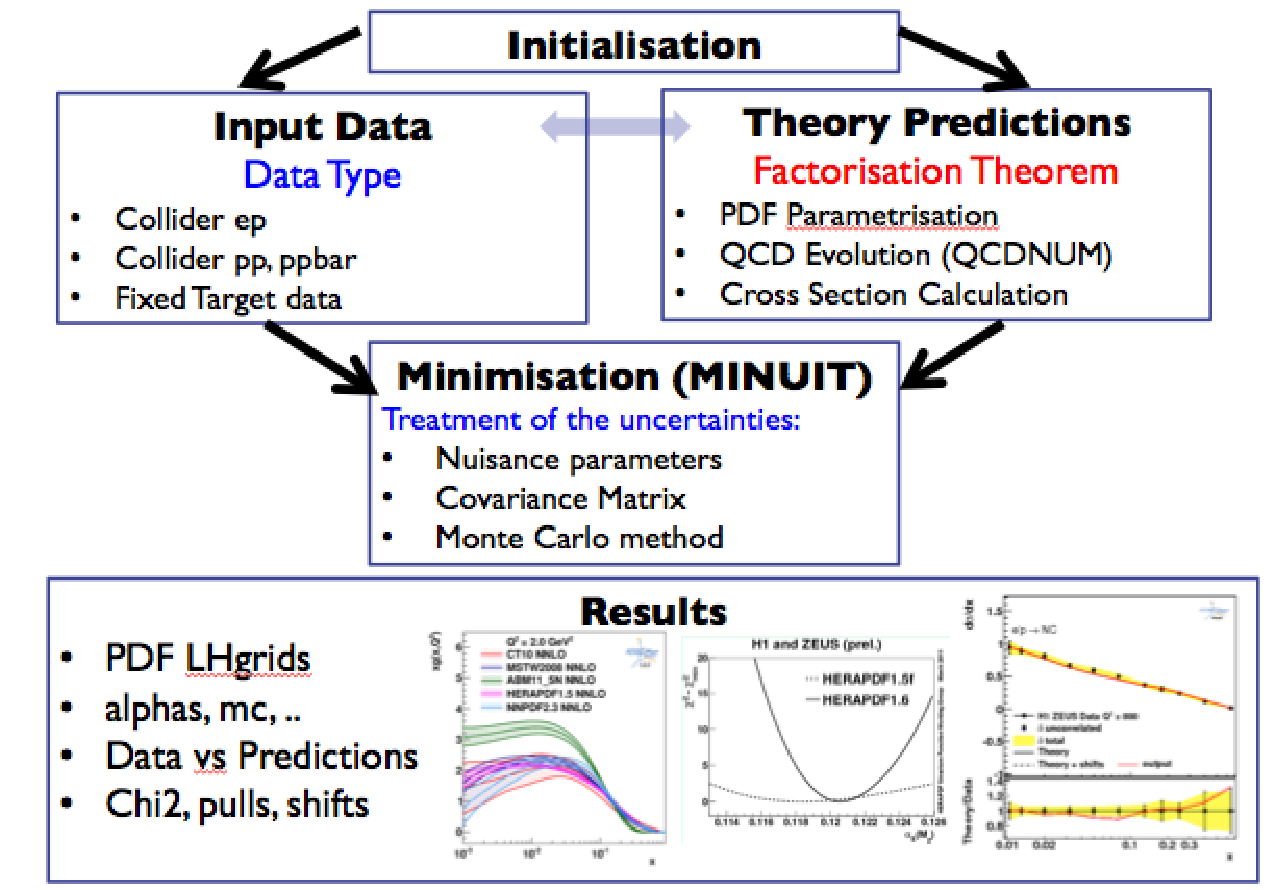
\includegraphics[width=8cm]{flow.pdf}
%   \caption{Schematic structure of the \fitter~program.} 
% \label{fig:flow}
%\end{figure}
\begin{description}
\item 
\bf {Input data:} \rm  All relevant cross section measurements from the various processes
are stored internally in \fitter with the full information on their uncorrelated and correlated
uncertainties. HERA I data sets are the basis of any proton PDF extraction, 
and they are used by all global PDF groups \cite{MSTWpdf, CT10pdf, NNPDFpdf, ABMpdf, JRpdf}. 
Additional measurements provide constraints to the sea flavour decomposition (such as the new 
results from the LHC), as well as constraints to PDFs in the kinematic phase-space regions 
where HERA data is not measured precisely, such as the high $x$ region for the gluon and valence quark distributions.
\item
\bf{Theory predictions:} \rm  Predictions for cross section of different processes are obtained using the factorisation approach (Eq.~\ref{eq:fact}). PDFs are parametrised at a starting scale $Q_0^2$  by a chosen functional form with a set of free parameters $\vec{p}$. These PDFs are then evolved from $Q_0^2$ to the scale of the measurement using the 
Dokshitzer-Gribov-Lipatov-Altarelli-Parisi 
(DGLAP)~\cite{Gribov:1972ri, Gribov:1972rt, Lipatov:1974qm,
Dokshitzer:1977sg, Altarelli:1977zs} evolution equations 
(as implemented in \qcdnum~\cite{qcdnum}), 
CCFM~\cite{\CCFM} or dipole models~\cite{Golec-Biernat:1998js,Iancu:2003ge,Bartels:2002cj} 
and then convoluted with the hard parton cross sections calculated
using a relevant theory program (as listed in Tab.~\ref{tab:proc}).
\item
\bf{PDF fit:} \rm  PDFs are extracted from a least square fit by constructing a 
$\chi^2$ from the input data and the theory prediction.
The $\chi^2$ is  minimized iteratively 
with respect to the PDF parameters using the MINUIT~\cite{minuit} program.
Various choices of accounting for the experimental uncertainties are employed in \fitter, either using 
a nuisance parameter method for the correlated systematic uncertainties, 
or a covariance matrix method (see details in section~\ref{sec:chi2representation}). In addition, \fitter allows to study different statistics 
assumptions for the distributions of the systematic uncertainties (i.e. Gauss or log-normal)~\cite{hera-lhc:report2009}.
%
In the $\chi^2$ minimization,
The parameters $\vec{p}$ of the parametrised PDFs and their uncertainties are extracted from the minimization fit.
%Fitted values of $\vec{p}$ and estimated uncertainties are obtained.
%The fitted parameters $\vec(p)$ and obtained from the uncertainties of the parameters are determined (from chi2+1???)
%
\item
\bf{Results:} \rm 
%The fitted parameters $\vec{p}$ and their estimated uncertainties are produced. 
The resulting PDFs are provided in a format ready to be used by the \lhapdf 
library~\cite{lhapdf,lhapdfweb} or by \tmdlib \cite{tmdlref}.
\fitter drawing tools can be used to display the PDFs with the uncertainty at a chosen scale.  
%Drawing tools are supplied which allow the PDFs to be
%graphically  displayed at chosen scales by the users with their one sigma uncertainty bands. 
A first set of PDFs extracted by \fitter is HERAPDF1.0 \cite{h1zeus:2009wt} (Fig.~\ref{fig:hera1}) 
which is based on HERA~I data.
Since then several other PDF sets were produced within the HERA and LHC collaborations.
In addition to PDF display, 
the figures comparing the data used in the fit and the relevant theory predictions are produced. 
% plots which compare the input data to the fitted theory predictions can be produced 
%to demonstrate the fit consistency. 
\begin{figure}[!ht]
   \centering
   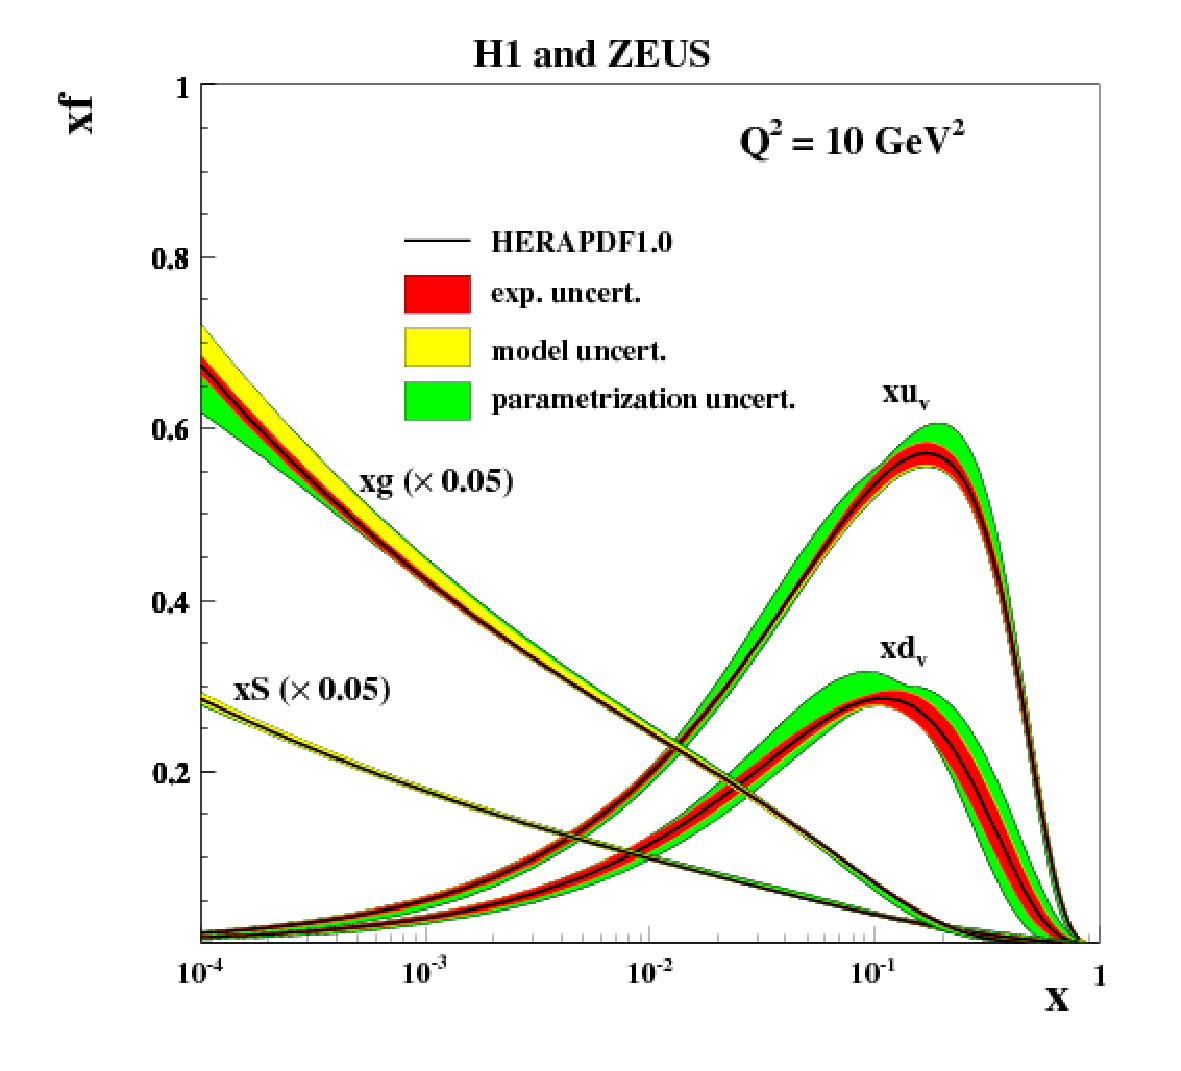
\includegraphics[width=8cm]{hera1.pdf}
   \caption{Summary plots of valence, total sea (scaled) and gluon densities (scaled) with their experimental, model and parametrisation uncertainties at the scale of $Q^2=10 \ \GeV^2$ for the HERAPDF1.0 PDF set at NLO~\cite{h1zeus:2009wt}.}
 \label{fig:hera1}
\end{figure}
In Fig.~\ref{fig:data}, a comparison of inclusive NC data from the HERA~I running period with predictions based on HERAPDF1.0. It also illustrates the comparison to the theory predictions which are adjusted by the  
systematic uncertainty shifts when using the nuisance parameter method that accounts for 
correlated systematic uncertainties. 
As an additional consistency check between data and the theory predictions, pull information, defined as the difference between data and prediction divided by the uncorrelated uncertaintly of the data, is displayed in units of sigma shifts for each given data bin.
% related only to the uncorrelated part of the systematic uncertainty. 

\begin{figure}[!ht]
   \centering
   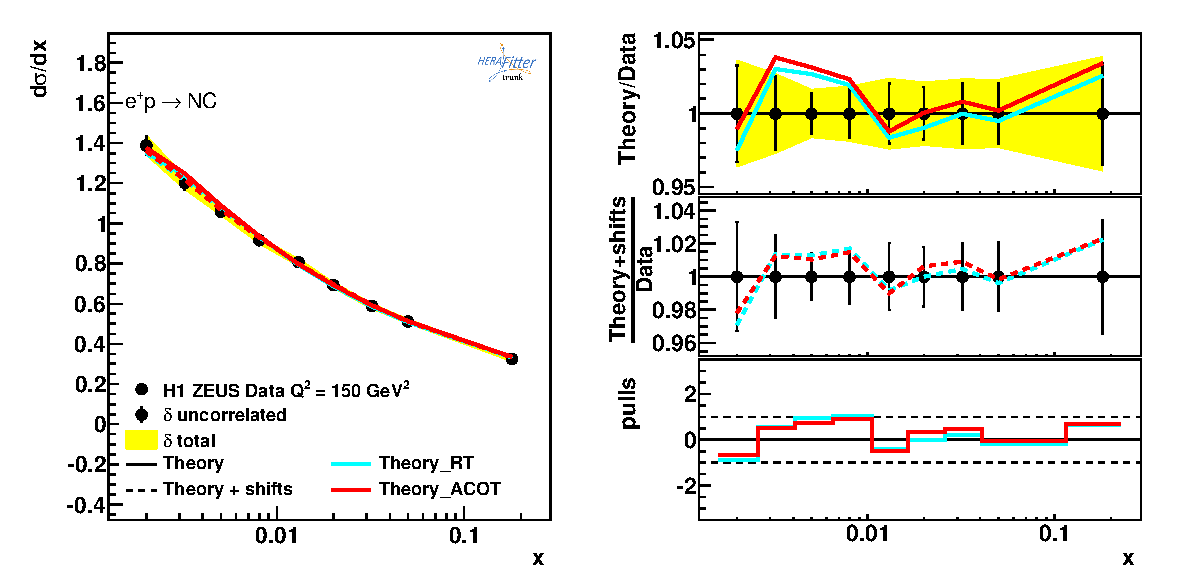
\includegraphics[width=8.6cm]{datatheory.pdf}
   \caption{An illustration of the \fitter drawing tools comparing the measurements (in the case of HERA I) to the predictions of the fit. In addition, ratio plots are also provided together with the pull distribution (right panel).} 
 \label{fig:data}
\end{figure}

\end{description}
%
%This paper provides a comprehensive description of  \\
%the \fitter\ package.
%which is designed for analysis of the High Energy Physics data.
%The package has been developed by members of the H1 and ZEUS collaborations
%with an exclusive support of different theoretical groups.
%The main purpose of the \fitter\ package is analysis of the 
%data from the $e^{\pm}p$, $p\bar{p}$, and $pp$ collider experiments
%information obtained from the deep inelastic scattering experiments
%and the determination of the parton density functions (PDFs).
%The broad range of data taken from the $e^{\pm}p$, $p\bar{p}$, and $pp$ collider experiments can be
%studied by the package. 

%Based on the concept of factorisable nature of the cross sections into universal parton distribution functions (PDFs) and process dependent partonic scattering cross sections, 

%The \fitter\ program facilitates the determination of the PDFs from many 
%cross section measurements at $ep$, $p\bar{p}$ or $pp$ colliders.  
% It includes various options for theoretical calculations and various choices 
%of how to 
%account for the experimental uncertainties. 
The \fitter project provides a versatile environment for benchmarking studies 
and a flexible platform for the QCD interpretation of analyses within the LHC experiments,
as already demonstrated by several publicly available results using the \fitter framework~\cite{atlas:strange,atlas:jets,atlas:hm,cms:strange,cms:jets,h1:2012kk,h1zeus:charm}.  

The outline of this paper is as follows.
%
Section~\ref{sec:theory} discusses the various processes 
and corresponding theoretical calculations performed in the DGLAP~\cite{Gribov:1972ri,Gribov:1972rt,Lipatov:1974qm,
Dokshitzer:1977sg,Altarelli:1977zs} formalism that are available in \fitter.
%
Section~\ref{sec:techniques} presents various techniques employed by the theory calculations used in \fitter.
Section~\ref{sec:method} elucidates the 
methodology of determining PDFs through fits based on various
% {\bf (what do you mean here
%by approaches?)} 
 $\chi^2$ definitions used in the
minimisation procedure. 
Alternative approaches to the DGLAP formalism are presented in section~\ref{sec:alternative}.
%
Specific applications of the package are given in
section~\ref{sec:examples}. 
%
%{\bf add something more here?.}

%
\section{Theoretical Input}
\label{sec:theory}
%
\subsection{Evolution}

\label{sec:evolution}
The \fitter\ program uses DGLAP~\cite{Gribov:1972ri,Gribov:1972rt,Lipatov:1974qm,Dokshitzer:1977sg,Altarelli:1977zs}
 evolution 
equations as implemented in the QCDNUM~\cite{qcdnum} program. The fit 
procedure begins with parameterising the input PDFs at the starting 
scale $Q^2_0$ which should be chosen to be below the charm mass threshold
$m_C^2$.
The PDFs are then evolved using the DGLAP evolution equations  
at NLO~\cite{Curci:1980uw,Furmanski:1980cm} in the $\overline{MS}$ scheme.
The renormalisation and factorisation scales are set to $Q^2$. The \fitter\ program
also allows for LO and NNLO evolution. 

The cross-section predictions are obtain by convoluting the PDFS with the 
coefficient functions. For the DIS processes, those are calculated 
using the general mass variable-flavour scheme. 
The program implements the  zero mass scheme from QCDNUM as well as
the RT scheme~\cite{Thorne:1997ga,Thorne:2006qt}. The jet cross sections
are calculated using APPLGRID and FastNLO. The program has two implementations
for $pp$  DY processes. The first implementation uses
calculations at LO which can be extended to NLO using k-factors,
the second uses the APPLGRID interface.
 
%\subsection{Coupling}
%\input{coupling}
\subsection{PDF parametrization}

\label{sec:pdf}
The parton density functions are parametrised at the starting scale by two formulae.
The first one is the standart HERA parametrization
\begin{equation}
xf(x)=A x^{B} (1-x)^{C} (1+Dx+Ex^{2}+Fx^{3}) - A_{\mathbf{p}} x^{B_{\mathbf{p}}} (1-x)^{C_{\mathbf{p}}}
\label{pdf:herapara}
\end{equation}
and the second one is the parametrization used by CTEQ collaboration
\begin{equation}
xf(x)=A x^{B} (1-x)^{C} e^{Dx} (1+e^{E}x+e^{F}x^{2}).
\label{pdf:ctpara}
\end{equation}
These formulas are used for parametrization of the gluon distribution $xg$,
the valence quark distributions $xu_{v}$,$xd_{v}$,
and the $u$-type and $d$-type anti-quark distributions $x\bar{U}$, $x\bar{D}$.
Here $x\bar{U}=x\bar{u}$, $x\bar{D}=x\bar{d}+x\bar{s}$ at the starting scale.

By default, HERA parametrization fits include 10 or 13 free parameters.
The resulting parametrization with 10 parameters is presented by the formulae
\begin{eqnarray}
\begin{array}{c}
xg(x)=A_{g} x^{B_{g}} (1-x)^{C_{g}}, \\
xu_{v}(x)=A_{u_{v}} x^{B_{u_{v}}} (1-x)^{C_{u_{v}}} (1+E_{u_{v}}x), \\
xd_{v}(x)=A_{d_{v}} x^{B_{d_{v}}} (1-x)^{C_{d_{v}}}, \\
x\bar{U}(x)=A_{\bar{U}} x^{B_{\bar{U}}} (1-x)^{C_{\bar{U}}}, \\
x\bar{D}(x)=A_{\bar{D}} x^{B_{\bar{D}}} (1-x)^{C_{\bar{D}}}.
\end{array}
\end{eqnarray}
Here the parameters
\begin{eqnarray}
\begin{array}{c}
B_{u_{v}}=B_{d_{v}}, \\
B_{\bar{U}}=B_{\bar{D}},\\
A_{\bar{U}}=A_{\bar{D}}\frac{1-f_{s}}{1-f_{charm}},
\end{array}
\end{eqnarray}
and coefficients $A$ are defined by the quark number and momentum sum-rules
\begin{eqnarray}
\begin{array}{c}
\int\limits_{0}^{1} u_{v}(x) dx =2, \\
\int\limits_{0}^{1} d_{v}(x) dx =1, \\
\int\limits_{0}^{1} x \left( g(x)+u(x)+\bar{u}(x)+d(x)+\bar{d}(x) \right) dx =1. \\
\end{array}
\end{eqnarray}
The strange quark distribution is fixed by $x$-independent fraction, $f_{s}$,
of the d-type sea, $x\bar{s}=f_{s}x\bar{D}$ at $Q_{0}^{2}$.

In case of 13 free parameters, the gluon formula is changed to
\begin{equation}
xg(x)=A_{g} x^{B_{g}} (1-x)^{C_{g}} - A_{\mathbf{p}g} x^{B_{\mathbf{p}g}} (1-x)^{C_{\mathbf{p}g}},
\label{pdf:herag13par}
\end{equation}
and parameters $A_{\mathbf{p}g}$, $B_{\mathbf{p}g}$, and $B_{d_{v}}$ are freed.

\subsection{$\chi^2$ Definition}
%%%%%%%%%%%%%%%%%%%%%%%%%%%%%%
\section{$\chi^2$ Definitions}
\label{sec:chi2}
%%%%%%%%%%%

For a single data set with diagonal statistical uncertainties, 
 the $\chi^2$ function can be defined as~\cite{H1:2009bp}
%
\begin{equation}
 \chi^2_{\rm exp}\left(\boldsymbol{m},\boldsymbol{b}\right) = %\\
%~~~=
 \sum_i
 \frac{\left[m^i
- \sum_j \gamma^i_j m^i b_j  - {\mu^i} \right]^2}
{ \textstyle \delta^2_{i,{\rm stat}}\left(m^i -  \sum_j \gamma^i_j m^i b_j\right)+
\left(\delta_{i,{\rm uncor}}\,  m^i\right)^2}
 + \sum_j b^2_j.
\label{eq:ave}\end{equation}
%
Here ${\mu^i}$ is the  measured central value  at a point $i$ 
with  relative statistical $\delta_{i,stat}$ 
and relative uncorrelated systematic uncertainty $\delta_{i,unc}$.
Further, $b_j$ denotes a nuisance parameter for
 a correlated systematic error  source of type $j$ with an uncertainty
 while
$\gamma^i_j$ 
quantifies the sensitivity of the
measurement ${\mu^i}$ at the point $i$ to the systematic source $j$. 
The function $\chi^2_{\rm exp}$ depends on the predicted values $m^i$ 
(denoted as the vector $\boldsymbol{m}$) and 
 the set of systematic uncertainties $b_j$ ($\boldsymbol{b}$).
The predicted values $m^i$ depend on the PDFs as well as other input
paremeter (e.g value of $\alpha_S$),  $m^i( \boldsymbol{p})$. 
In the following, absolute (relative) values of uncertainties are given
by capital (small) Greek symbols, e.g. $\Delta^i_{\rm stat}$ ( $\delta^i_{\rm stat} )$. 

This definition of the $\chi^2$ function assumes that
systematic uncertainties are proportional to the central values 
(multiplicative errors), whereas the statistical errors scale 
with the square roots of the expected number of events. 
Other scaling properties for the statistical and uncorrelated
systematic uncertainties are discussed later.
% available as described in appendix~\ref{sec:herafitter}.
%%%%

In the case of off-diagonal statistical uncertainties, the $\chi^2$ function
is
\begin{equation} \label{eq:chi2gen}
\chi^2_{\rm exp} (\boldsymbol{m},\boldsymbol{b}) = \sum_{ij} \left ( m^i - \sum_l \Gamma^i_l(m^i)b_l - \mu^i \right)
  C^{-1}_{{\rm stat.}~ij}(m^i,m^j) \left(  m^j - \sum_l \Gamma^j_l(m^j)b_l - \mu^j \right) + 
\sum_l b^2_l \,.
\end{equation}
Here the scaling properties of the correlated systematic uncertainties 
$\Gamma^i_j$ and
of the covariance matrix $C_{{\rm stat.}~ij}$ are expresses as a dependence
on $m_i$ and the dependence of $\Delta_{\rm stat}$ on $b_j$ is ignored.

Eq.~\ref{eq:chi2gen} allows for two methods for fast determination
of the minimum, without need to include the formal nuisance parameters
corresponding to the systematic error sources into the minuit minimisation.
In the first method, the minimisation vs. $b_j$ is used to define covariance
matrix for the systematic uncertainties which is determined as
\begin{equation}
 C_{{\rm syst}~ij}= \sum_l \Gamma^i_l \Gamma^j_l \,.
\end{equation}
The total covariance matrix is given by the sum of the statistical and
systamtic covariance matrices
\begin{equation} 
C_{{\rm tot}~ij} = C_{{\rm stat}~ij} + C_{{\rm syst}~ij}\,,
\end{equation}
and the $\chi^2$ function takes a form
\begin{equation}
  \chi^2( \boldsymbol{m}) = \sum_{ij} ( m^i - \mu^i) C^{-1}_{{\rm tot}~ij} 
( m^j - \mu^j)\,.
\end{equation}

The second methods is used to determine optimal shifts of the nuisance
parameters at each iteration. The shifts are given by minimising 
Eq.~\ref{eq:chi2gen} vs. $b_j$ which leads to a system of  linear equations 
\begin{equation}
 \sum_k \sum_{ij} C^{-1}_{{\rm stat}~ij} \Gamma^i_l \Gamma^j_k \cdot b_k = \sum_{ij} C^{-1}_{{\rm stat}~ij} \Gamma^i_l (m_i - \mu_i)\,,
\end{equation}
where $1\le l \le N_{\rm syst}$, the total number of correlated systematic uncertainties.

Finally the nuisance parameters $\boldsymbol{b}$ can be excluded from the $\chi^2$ minimisation.  
In this case, which is referred to as an Offset method, the minimum is determined for their values set to zero
while uncertainties on the parameters $\boldsymbol{p}$ are determined by shifting each nuisance parameter $b_l$
by $\pm 1$. The total covariance matrix for parameters $p^i$ is determined as 
\begin{equation}
  C^{\rm offset}_{ {\rm par}~ ij} = \sum_{l=1}^{N_{syst}} \Delta p^i_l \Delta p^j_l \,,
\end{equation}
where $ \Delta p^i_l = 0.5 ( p^i( b_l = +1 ) - p^i(b_l = -1))$ and the quality of the fit is estimated by 
fixing $\boldsymbol{p}$ to the value at the minimum and minimising with respect to $\boldsymbol{b}$

Finally, all three approaches can be combined together. For example, only some of the systematic uncertainties
can be treated using the matrix method while others can be treated using the hessian method. In this case, the
covariance matrix  $C_{\rm syst}$ is build using the corresponding sub-set of systematic sources and $C_{\rm stat}$ 
is replaced by $C_{\rm stat}+C_{\rm syst}$ in Eq.~\ref{eq:chi2gen}. Similarly, some of the systematic uncertainties
can be treated using offset method and then $C^{\rm total}_{ {\rm par}} = C^{\rm hessian}_{\rm par} + C^{\rm offset}_{\rm par}$
where offset and hessian covariance matrices are calculated using corresponding systematic error sources.

\subsection{Bias corrections}

The correlated and uncorrelated systematic uncertainties can be treated as additive,  $\Gamma^i_l(m^i) = \gamma^i_l \mu^i$
or multiplicative, $\Gamma^i_l(m^i) = \gamma^i_l m^i$. The LogNormal treatment in which 
$ \mu^i + \sum_l \Gamma^i_j b_l$ is replaced by $ \mu^i \prod_l \exp( \gamma^i_j b_l) $ is forseen for the
next release of the {\tt HERAFitter}. 

The statistical uncertainties can be treated as additive, $\Delta^i(m^i) = \delta^i \mu^i$  and as Poisson,
$\Delta^i(m^i) = \delta^i \sqrt{\mu^i m^i}$. More complex scaling from Eq.~\ref{eq:ave}, 
which depends on shifts of $b_j$, is implemented using an iterative approach: for the first iteration $b_l =0$ 
 is used to determine values of $b_l$ which are then applied in the second iteration. Statistical covariance
matrix is scaled in a similar manner. In this case the correlation matrix is assumed to be fixed, the diagonal
ellements are updated using the prescription describe above and the covariance matrix is rescaled accordingly.

The modifications of the covariance matrix at each iteration of the minuit minimisation may lead to systematic
biases. There are two approaches to avoid these biases. In the first approach the covariance matrix is calculated
using the expected values at the first iteration of the minimisation and kept fixed to these values for further
iterations. This method requires several repetitions of the minimisation, to ensure that values close to optimal
are obtained already at the first iteration. The second method modifies the $\chi^2$ function by adding a term
corresponding to non-constant value of the covariance matrix:
\begin{equation}
 \chi^2_{\rm log} = 2 \log \frac{\Delta^i(m^i)}{\Delta^i(\mu^i)} 
\end{equation}  

\subsection{HERAFitter implementation}

%%%%%%%%%%%
% \subsection{Using Covariance Matrix}
%%%%%%%%%%%%%%%%%%%%%%%%%%%%%
 
%
%
\section{Data}
\label{sec:data}
%
\subsection{Data Sets}

\label{sec:data}
The following datasets are used for fits...

%\subsection{Overview of Systematic Uncertainties}
%\input{systematics}
%\section{Fits}
%\label{sec:fits}
%\subsection{DGLAP Fit}
%\label{sec:qcdfit}
%\input{qcd}
%\subsection{Dipole Model Fits}
%\input{dipole}
%% no discussion ...
%% \subsection{Discussion of Fit Results}
%% \input{discussion}
%%\subsubsection{Framework and Parameterisations}
%%\input{qcdset}
%%\subsubsection{Results and Kinematic Cut Variations}
%%\input{qcdresult}
%%
%%\subsection{Discussion}
%%
\section{Summary}
\label{sec:conclusion}

\label{sec:summary}
\fitter is an open-source platform designed for studies of the structure of the proton.
It provides a unique and flexible framework with a wide variety of QCD tools to 
facilitate analyses of the experimental data and theoretical calculations. 
\fitter allows for direct comparisons of various theoretical approaches under the same settings,
different methodologies in treating the experimental and model uncertainties can be used for benchmarking studies.
The progress of \fitter is driven by the latest QCD advances in theoretical calculations and in the precision of experimental data.

The \fitter code, in version $1.1.0$, has sufficient options to reproduce the different theoretical choices made in MSTW, CTEQ and ABM fits. This will potentially make it a  
valuable tool for benchmarking and understanding differences between PDF fits. Such a study would however need to consider a range of further questions, such as the choices of
data sets, treatments of uncertainties, input parameter values, $\chi^2$ definitions and so forth. We look forward to studying these questions in future work.



%
\section*{Acknowledgements}
\refstepcounter{pdfadd} \pdfbookmark[0]{Acknowledgements}{s:acknowledge}
%\begin{theacknowledgments}    
%
We are grateful to the HERA machine group whose outstanding
efforts have made this experiment possible.
We thank the engineers and technicians for their work in constructing
and maintaining the H1 detector, our funding agencies for
financial support, the DESY technical staff for continual assistance
and the DESY directorate for support and for the hospitality
which they extend to the non DESY members of the collaboration.
%\end{theacknowledgments}


\bibliography{fitter.bib}  
\clearpage

%\input{tables}

%\clearpage

%\input{figures}


\end{document}

